\item Se o sistema é solto do repouso, determine a velocidade dos cilindros de \SI{20}{\kilogram}, $A$ e $B$, após $A$ ter se
deslocado para baixo uma distância de \SI{2}{\meter}. A polia diferencial tem massa de \SI{15}{\kilogram} e raio de giração
em relação a sua centro de massa $k_{O}=\SI{100}{\milli\meter}$.

\import{../answers}{answer-4}

\vspace{-1.5cm}
\begin{flushright}
	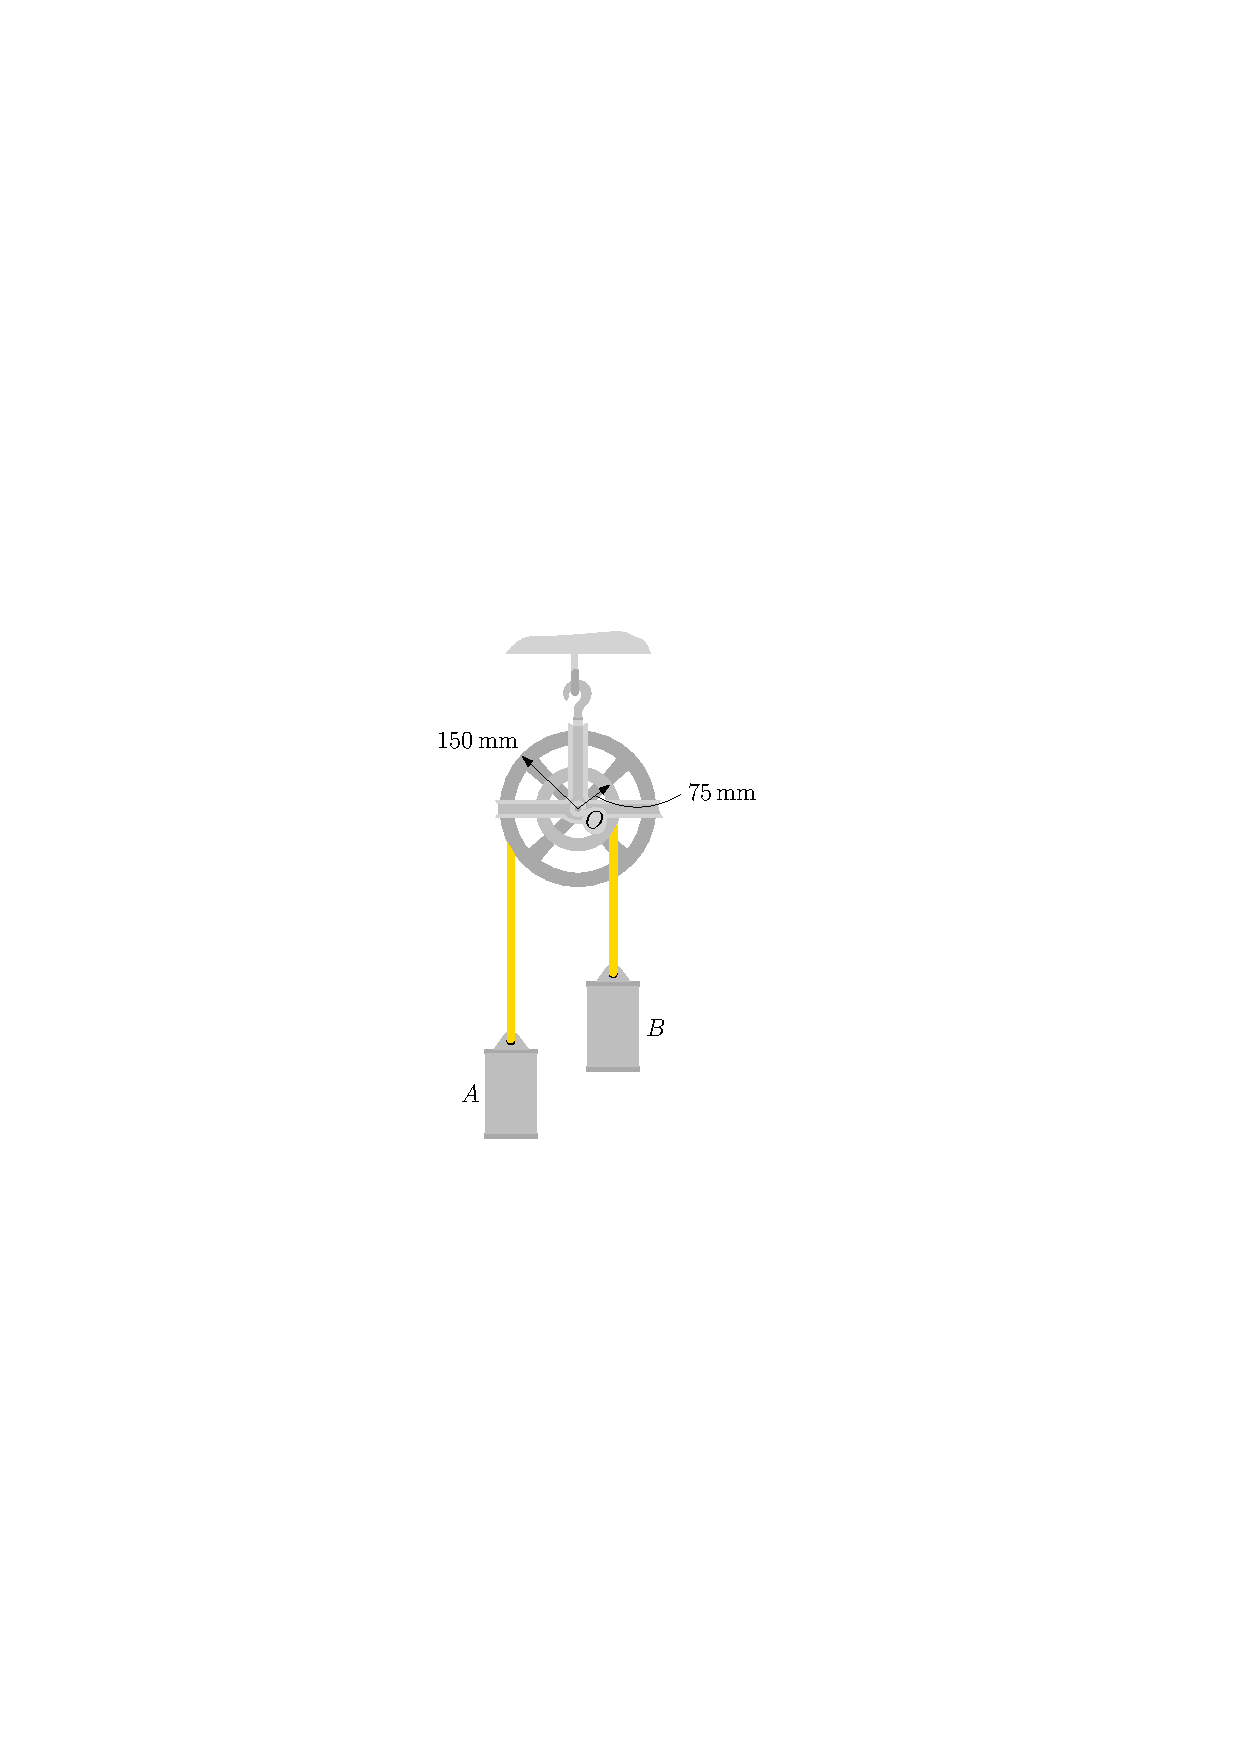
\includegraphics[scale=1.]{../../images/draw_3}
\end{flushright}